\documentclass{beamer}
\usepackage{fancybox}
\usepackage{tikz}
\usetikzlibrary{arrows.meta,
                chains,
                positioning, 
                shadows.blur, shapes.arrows}

\usepackage{amsmath}              
\usepackage{mathabx}

\usetheme{Madrid}
\newcommand{\G}{\mathcal{G}}

\title{Logic Tensor Networks}

\author{Robert Hoehndorf}
\date{\today}

\begin{document}

\frame{\titlepage}

\begin{frame}
  \frametitle{Introduction}
  \begin{itemize}
  \item Logic Tensor Networks (LTN) is neuro-symbolic framework based
    on fuzzy differentiable logic
  \item Supports tasks based on manipulating data and knowledge
  \item It has been shown to effectively tackle many tasks that are
    central to intelligent systems:
    \begin{itemize}
    \item multi-label classification,
    \item relational learning,
    \item data clustering,
    \item semi-supervised learning,
    \item regression,
    \item embedding learning, and
    \item query answering under uncertainty
    \end{itemize}
  \end{itemize}
\end{frame}

\begin{frame}
  \frametitle{Introduction}
  \begin{itemize}
  \item use of infinitely-valued fuzzy logic (Real Logic)
  \item domains are interpreted as tensors in the Real field
  \item use ``grounding'' instead of ``interpretation''
  \end{itemize}
\end{frame}

\begin{frame}
\frametitle{Real Logic in Logic Tensor Networks}
\begin{itemize}
    \item Real Logic is based on a first-order language \( L \)
    \item Includes constant symbols (\( C \)), functional symbols (\(
      F \)), relational symbols (predicates, \( P \)), and variable
      symbols (\( X \))
    \item Facilitates the expression of relational knowledge with variables
      \begin{itemize}
      \item first order logic
      \end{itemize}
\end{itemize}
\end{frame}

\begin{frame}
\frametitle{Atomic Formulas and Fuzzy Semantics}
\begin{itemize}
    \item Atomic formula example: \( \text{is\_friend}(v1, v2) \)
    \item Symmetric relations example: \( \forall x \forall y
      (\text{is\_friend}(x, y) \Rightarrow \text{is\_friend}(y, x))
      \)
    \item Incorporates fuzzy semantics for partial truth in real-world
      scenarios
\end{itemize}
\end{frame}

\begin{frame}
\frametitle{Types and Domain Assignment}
\begin{itemize}
    \item Domains assigned using functions \( D, D_{in}, \) and \( D_{out} \)
    \item \( D \): Assigns domains to variables and constants
    \item \( D_{in} \) and \( D_{out} \): Define input and output domains
      for functions and predicates
\end{itemize}
\end{frame}

\begin{frame}
\frametitle{Terms and Formulas in Real Logic}
\begin{itemize}
    \item Terms formed from constants, variables, and function symbols
    \item Formulas include atomic formulas, expressions with
      connectives, and quantified expressions
    \item Supports negation, conjunction, disjunction, implication,
      and biconditional, as well as universal and existential
      quantifiers
\end{itemize}
\end{frame}

\begin{frame}
\frametitle{Example of Real Logic Application}
\begin{itemize}
    \item Domains (types): \( \text{Town} \) and \( \text{People} \)
    \item Constants like Alice, Bob (People) and Rome, Seoul (Town)
    \item Example of well-formed expression: \(
      \text{lives\_in}(\text{Alice}, \text{Rome}) \) 
    \item Example of malformed expression: \(
      \text{lives\_in}(\text{Bob}, \text{Charlie}) \)
\end{itemize}
\end{frame}

\begin{frame}
  \frametitle{Semantics}
  \begin{itemize}
  \item Domains are interpreted concretely by tensors in the Real
    field
  \item tensors are algebraic objects that include
    \begin{itemize}
    \item Scalars: 0-dimensional
    \item Vectors: 1-dimensional,
    \item Matrices: 2-dimensional,
    \item as well as higher-dimension structures
    \end{itemize}
  \item To emphasize this, the authors use the term ``grounding'',
    denoted with the letter $\G$, instead of
    ``interpretation'' (the usual name for this concept in logic)
  \end{itemize}
\end{frame}

\begin{frame}
  \frametitle{Semantics}
  Grounding $\mathcal{G}$ maps
  \begin{itemize}
  \item Terms to tensors of real numbers
  \item Formulas to real numbers in the interval [0,1]
  \end{itemize}
\end{frame}

\begin{frame}
  \frametitle{Variables and constants}
  \begin{itemize}
  \item Constants:
    \begin{itemize}
    \item Denote individuals from a space of tensors of any rank:
    \item The individual can be pre-defined (data point) or learnable
      (embedding)
    \item Intuition: Each dimension corresponds to a feature, and the
      number corresponds to the value of that feature for that
      individual
    \end{itemize}
  \item Variables denote sequences of individuals:
    \begin{itemize}
    \item Sequences represent the possible values that the variable can take
    \item They can contain more than one instance of the same value
    \end{itemize}
  \end{itemize}
\end{frame}

\begin{frame}
\frametitle{Functions}
\begin{itemize}
    \item Functions can be any mathematical function, either
      pre-defined or learnable
    \item Examples of functions include distance functions,
      regressors, etc.
\end{itemize}
\end{frame}

% Slide 2: Predicates
\begin{frame}
\frametitle{Predicates}
\begin{itemize}
    \item Represented as mathematical functions mapping an n-ary
      domain of individuals to a real number in \([0,1]\), interpreted
      as a truth degree
    \item Examples of predicates include similarity measures,
      classifiers, etc.
\end{itemize}
\end{frame}

% Slide: Definition 2
\begin{frame}
\frametitle{Definition 2: Grounding in Real Logic}
\begin{block}{Grounding \( \G \) of \( L \)}
A grounding $\G$ of \( L \) is a function defined on the signature of \( L \) that satisfies the following conditions:
\begin{enumerate}
    \item \( \G(x) = \langle d_1, \ldots, d_k \rangle \in
      \bigtimes_{i=1}^{k} G(D(x)) \) for every variable symbol \( x
      \in X \), with \( k \in \mathbb{N}_0 \). \( \G(x) \) is a
      sequence, not a set, allowing multiple occurrences of the same
      value from \( \G(D(x)) \)
    \item \( \G(f) \in \G(D_{\text{in}}(f)) \rightarrow
      \G(D_{\text{out}}(f)) \) for every function symbol \( f \in F
      \)
    \item \( \G(p) \in \G(D_{\text{in}}(p)) \rightarrow [0, 1] \) for
      every predicate symbol \( p \in P \)
\end{enumerate}
\end{block}
\end{frame}

\begin{frame}
  \frametitle{Example}
  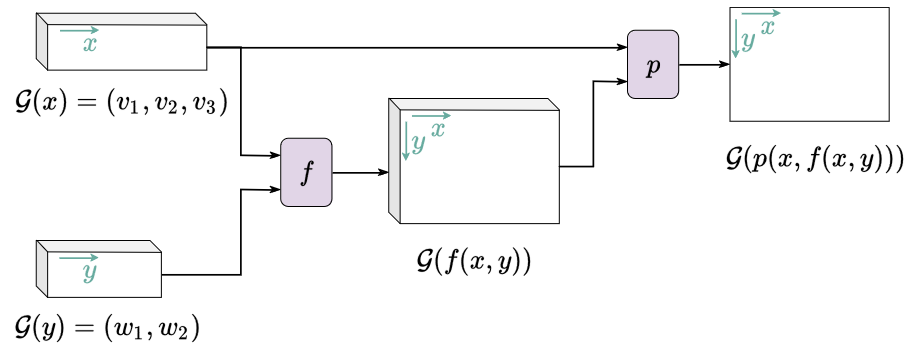
\includegraphics[width=\textwidth]{ltn1.png}
  % Page 7 of LTN Arxiv paper, Example 3
\end{frame}

\begin{frame}
  \frametitle{Connectives}
  Connectives are modeled using fuzzy semantics:
  \begin{itemize}
  \item conjunction: t-norm
  \item disjunction: t-conorm
  \item negation: fuzzy negator
  \item implication: fuzzy implication
  \end{itemize}
  Quantifiers are defined using aggregators (symmetric and continuous
  operators)
  \begin{itemize}
  \item Existential ($\exists$): Generalization of existential quantification in FOL
  \item Universal ($\forall$): Generalization of universal quantification in FOL
  \end{itemize}
\end{frame}

% Slide 1: Table 1 - The t-norms of interest
\begin{frame}
\frametitle{Table 1: The t-norms of Interest}
\resizebox{\textwidth}{!}{
\begin{tabular}{l|l|l}
\textbf{Name} & \textbf{T-norm} & \textbf{Properties} \\
\hline
Gödel (minimum) & \(T_G(a, b) = \min(a, b)\) & idempotent, continuous \\
Product & \(T_P(a, b) = a \cdot b\) & strict \\
Łukasiewicz & \(T_{LK}(a, b) = \max(a + b - 1, 0)\) & continuous \\
Drastic product & \(T_D(a, b) = 
\begin{cases}
\min(a, b), & \text{if } a = 1 \text{ or } b = 1 \\
0, & \text{otherwise}
\end{cases}\) &  \\
Nilpotent minimum & \(T_{nM}(a, b) = 
\begin{cases}
0, & \text{if } a + b \leq 1 \\
\min(a, b), & \text{otherwise}
\end{cases}\) & left-continuous \\
Yager & \(T_Y(a, b) = \max(1 - ((1 - a)^p + (1 - b)^p)^{\frac{1}{p}}, 0), p \geq 1\) & continuous \\
\end{tabular}
}
\end{frame}

% Slide 2: Table 2 - The t-conorms of interest
\begin{frame}
\frametitle{Table 2: The t-conorms of Interest}
\resizebox{\textwidth}{!}{
\begin{tabular}{l|l|l}
\textbf{Name} & \textbf{T-conorm} & \textbf{Properties} \\
\hline
Gödel (maximum) & \(S_G(a, b) = \max(a, b)\) & idempotent, continuous \\
Product (probabilistic sum) & \(S_P(a, b) = a + b - a \cdot b\) & strict \\
Łukasiewicz & \(S_{LK}(a, b) = \min(a + b, 1)\) & continuous \\
Drastic sum & \(S_D(a, b) = 
\begin{cases}
\max(a, b), & \text{if } a = 0 \text{ or } b = 0 \\
1, & \text{otherwise}
\end{cases}\) &  \\
Nilpotent maximum & \(S_{nM}(a, b) = 
\begin{cases}
1, & \text{if } a + b \geq 1 \\
\max(a, b), & \text{otherwise}
\end{cases}\) & right-continuous \\
Yager & \(S_Y(a, b) = \min((a^p + b^p)^{\frac{1}{p}}, 1), p \geq 1\) & continuous \\
\end{tabular}
}
\end{frame}

% Slide: Common Aggregation Operators
\begin{frame}
\frametitle{Common Aggregation Operators}
\resizebox{\textwidth}{!}{%
\begin{tabular}{|l|l|l|}
\hline
\textbf{Name} & \textbf{Generalizes} & \textbf{Aggregation Operator} \\
\hline
Minimum & \( T_G \) & \( A_{T_G}(x_1, \ldots, x_n) = \min(x_1, \ldots, x_n) \) \\
\hline
Product & \( T_P \) & \( A_{T_P}(x_1, \ldots, x_n) = \prod_{i=1}^{n} x_i \) \\
\hline
Łukasiewicz & \( T_{LK} \) & \( A_{T_{LK}}(x_1, \ldots, x_n) = \max\left(\sum_{i=1}^{n} x_i - (n - 1), 0\right) \) \\
\hline
Maximum & \( S_G \) & \( E_{S_G}(x_1, \ldots, x_n) = \max(x_1, \ldots, x_n) \) \\
\hline
Probabilistic sum & \( S_G \) & \( E_{S_P}(x_1, \ldots, x_n) = 1 - \prod_{i=1}^{n} (1 - x_i) \) \\
\hline
Bounded sum & \( S_{LK} \) & \( E_{S_{LK}}(x_1, \ldots, x_n) = \min \left(\sum_{i=1}^{n} x_i, 1\right) \) \\
\hline
\end{tabular}
}
\end{frame}

% Slide 1: Explanation of Types of Implication (S and R)
\begin{frame}
\frametitle{Types of Fuzzy Implications}
Fuzzy implications are functions \( I: [0, 1]^2 \to [0, 1] \) that are increasing with respect to the first argument and decreasing with respect to the second. They satisfy boundary conditions \( I(0, 0) = I(1, 1) = 1 \), and \( I(1, 0) = 0 \). Two classes of fuzzy implications are considered:
\begin{itemize}
    \item \textbf{S-implications}: Formed using a t-conorm and generalizing the material implication \( a \to c = \neg a \oplus c \).
    \item \textbf{R-implications}: Standard in t-norm fuzzy logics, constructed from t-norms.
\end{itemize}
\end{frame}

% Slide: S-implications
\begin{frame}
\frametitle{S-implications with Common t-Conorms}
\resizebox{\textwidth}{!}{%
\begin{tabular}{|l|l|l|l|}
\hline
\textbf{Name} & \textbf{T-conorm} & \textbf{S-implication} & \textbf{Properties} \\
\hline
Gödel (Kleene-Dienes) & \( S_G \) & \( I_{KD}(a, c) = \max(1 - a, c) \) & All but IP \\
Product (Reichenbach) & \( S_P \) & \( I_{RC}(a, c) = 1 - a + a \cdot c \) & All but IP \\
Łukasiewicz & \( S_{LK} \) & \( I_{LK}(a, c) = \min(1 - a + c, 1) \) & All \\
Dubouis-Prade & \( S_D \) & $I_{DP}(a, c) = 
\begin{cases} 
c, & \text{if } a = 1 \\
1 - a, & \text{if } c = 0 \\
1, & \text{otherwise}
\end{cases}$ & All \\
Nilpotent (Fodor) & \( S_{Nm} \) & $I_{FD}(a, c) = 
\begin{cases} 
1, & \text{if } a \leq c \\
\max(1 - a, c), & \text{otherwise}
\end{cases}$ & All \\
\hline
\end{tabular}%
}
\end{frame}

% Slide: Negators and De Morgan Triplets
\begin{frame}
\frametitle{Negators and De Morgan Triplets}
\begin{block}{Negator}
A negator \( n: [0, 1] \to [0, 1] \) is a monotonically decreasing mapping such that \( n(0) = 1 \) and \( n(1) = 0 \). It is:
\begin{itemize}
    \item Strict if it is strictly monotonically decreasing.
    \item Strong if it is strict and involutive, i.e., \( n(n(x)) = x \) for all \( x \in [0, 1] \).
\end{itemize}
The standard (canonical) negator is \( n(x) = 1 - x \), which is both strict and strong.
\end{block}

\begin{block}{De Morgan Triplet}
A De Morgan triplet is a triple \( (T, \perp, n) \) where:
\begin{itemize}
    \item \( T \) is a t-norm.
    \item \( \perp \) is a t-conorm according to the axiomatic definition of t-conorms.
    \item \( n \) is a strong negator.
    \item \( \forall a, b \in [0, 1] \): \( n(\perp(a, b)) = T(n(a), n(b)) \).
\end{itemize}
\end{block}
\end{frame}

\begin{frame}
  \frametitle{Conjunction}
  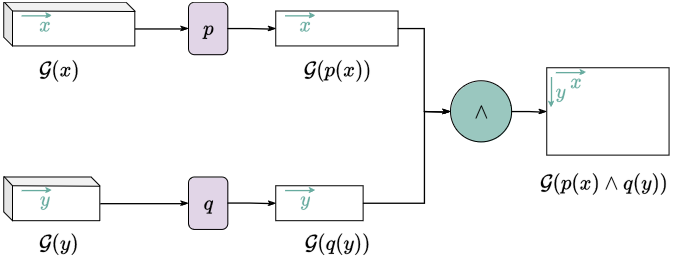
\includegraphics[width=\textwidth]{ltn2.png}
\end{frame}

\begin{frame}
  \frametitle{Quantification}
  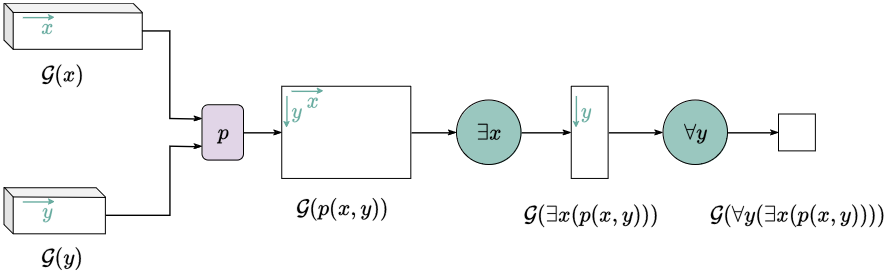
\includegraphics[width=\textwidth]{ltn3.png}
\end{frame}

% Slide: Diagonal Quantification in LTN
\begin{frame}
\frametitle{Diagonal Quantification in LTN}
\begin{block}{Diagonal Quantification (Diag)}
\begin{itemize}
    \item Diagonal quantification is denoted as \( \text{Diag}(x_1, \ldots, x_h) \).
    \item It quantifies over specific tuples such that the \( i \)-th tuple contains the \( i \)-th instance of each variable.
    \item Assumes all variables are grounded onto sequences with the same number of instances.
    \item Quantifies over the diagonal of \( G(\phi) \) along the axes associated with \( x_1 \ldots x_h \).
    \item Used for statements that hold true for each pair of sample and label, e.g., \( \forall\text{Diag}(x, y) p(x, y) \) for datasets with samples \( x \) and target labels \( y \).
    \item Reduces computational complexity by avoiding evaluation for all combinations in \( G(x) \) and \( G(y) \).
\end{itemize}
\end{block}
\end{frame}

\begin{frame}
  \frametitle{Diagonal quantification}
  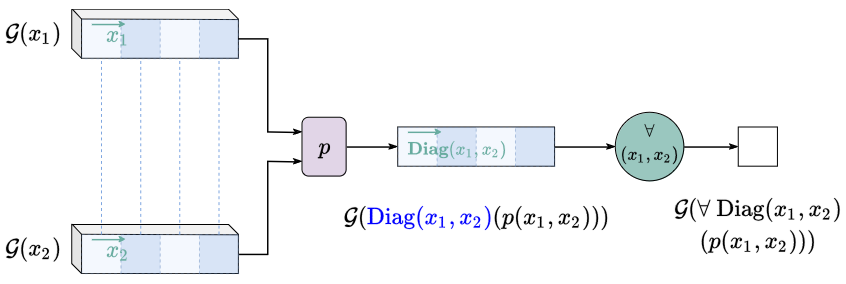
\includegraphics[width=\textwidth]{ltn4.png}
\end{frame}

% Slide: Quantification Over Domain Elements
\begin{frame}
\frametitle{Guarded quantification}
\begin{block}{Quantifying Based on a Condition}
In many situations, it's desirable to quantify over a set of elements
in a domain whose grounding satisfies a specific condition. For
example, one might express a condition using formulas like:
\begin{itemize}
    \item \( \forall y (\exists x : \text{age}(x) > \text{age}(y)) (\text{parent}(x, y)) \)
\end{itemize}
This formula aggregates values of the \textit{parent} predicate only for instances of \( x \) that satisfy the age condition with respect to \( y \).
\end{block}
\end{frame}

% Slide: Grounding Formulas with Conditional Aggregation
\begin{frame}
\frametitle{Grounding Formulas with Conditional Aggregation}
\begin{block}{Aggregating Values Based on Conditions}
The grounding of a formula like \( \forall y (\exists x: \text{age}(x) > \text{age}(y)) (\text{parent}(x, y)) \) involves:
\begin{itemize}
    \item Aggregating values of \( \text{parent}(x, y) \) only for instances of \( x \) that satisfy \( \text{age}(x) > \text{age}(y) \).
    \item Mathematically represented as:
\end{itemize}
\[
\text{Agg}({\forall})_{j=1}^{|\G(y)|} \text{Agg}({\exists})_{\substack{i=1 \\ \G(\text{age}(x))_i > \G(\text{age}(y))_j}}^{|\G(x)|} \G(\text{parent}(x, y))_{i,j}
\]
\end{block}
\end{frame}

\begin{frame}
\frametitle{Guarded Quantifiers and Symbolic Evaluation}
\begin{block}{Symbolic and Non-differentiable Evaluation}
The evaluation of whether a tuple is safe is symbolic and non-differentiable. Guarded quantifiers only operate over a subset of variables when crisp symbolic knowledge is available.
\end{block}

\begin{block}{Guarded Quantifiers with Masks}
Let \( m \) be a mask representing a condition, and \( \G(m) \) associates a Boolean function to \( m \). The grounding of a guarded quantifier is defined as:
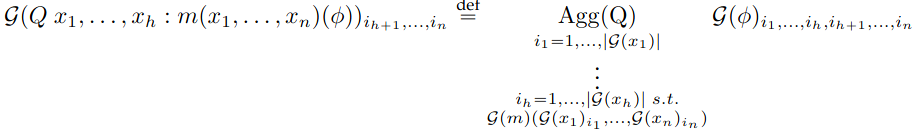
\includegraphics[width=\textwidth]{ltn5.png}
\end{block}
\end{frame}

\begin{frame}
  \frametitle{Guarded quantification}
  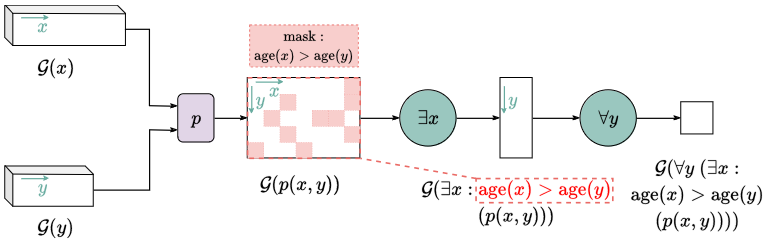
\includegraphics[width=\textwidth]{ltn6.png}
\end{frame}




\end{document}


%%% Local Variables:
%%% mode: latex
%%% coding: utf-8
%%% TeX-master: t
%%% eval: (TeX-run-style-hooks "beamer")
%%% End:
